\newpage
\chapter{Platform} \textit{Dennis}
\section{Environment}
The system is primarily to be used from the same PC, as the webpage is part of an energy system
placed at the school, AU Herning. A part of the energy system is a screen showing the webpage to
be able to control the system nearby it. The screens resolution is 1024x768 pixels (fullscreen with no system bars or dock), 
which is the size the site has been optimised for. Also the website has been optimised for small-screen devises with a resolution from 320x480 pixels (as this resolution has been used for several phones in the last years).
\section{File Structure}
The website can be found on http://www.ehub.threee.dk/, the file structure on the ftp server is as follow. In the index folder/root of the site, the folders: design, mobile, modules and pic can be found together with the .html files and .css files created for the index page. The root folder contains:
\begin{itemize}
	\item design: Photoshop files
	\item mobile: .html, .css and images used for the mobile site
	\item modules: .html and .css files for the module pages.
	\item pic: Icons and other pictures used on the site.	
	\item index.html
	\item reset.css + style\_index.css
\end{itemize}
In the modules folder is found the style sheet of the module pages and folders containing a html file for each module plus a special style sheet to setup the things inside the main window. The mobile folder contains a copy of the normal website in an optimised version.

\begin{figure}[htbp]
	\center
	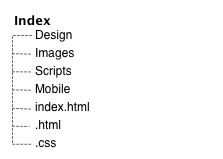
\includegraphics[width=0.75\textwidth]{images/hierarki.png} % requires the graphic package
   	\caption{Hierarchy of the files on the server}
   	\label{fig:file_hierarki}
\end{figure}
\newpage
\section{Image scaling}
To not scare away the user because of too long loading times, pictures putted on a webpage should be scaled and converted properly. To do so, some rules of thumb should be followed. An important factor is to scale the image in an image editor like Photoshop to a proper size. In other words, the image scaling should \textbf{not} be done by the web-browser. Another important thing is to analyse the content of the image to use the right image format and thereby convert the image to the optimal type for the place implemented.
\\The most used image formats on the internet is GIF, PNG and JPG/JPEG, where JPG/JPEG is mostly used for colourful images like photographies. For icons, pictures being part of the design and flat coloured images, should be used either GIF or PNG. When choosing between GIF and PNG some considerations should be taken, like: what browser uses the main audience, how should the pictures be shown and what colour debt is needed. For the website created the type PNG has been used for all graphics as the amount of colours needed was not full filed when the pictures was converted to GIF and the browsers for the user(s) of the website will primarily be non Internet Explorer. Internet Explorer older than version 9 unfortunately still has some problems with showing transparent PNG images which is used, but still the colour debt of the images was weighted higher than cross compatibility. Also an IE Javascript fix for the PNG transparency has been found, but yet not implemented as the goal so far has only been to write HTML and CSS code. 

\section{Reset.css} \textit{Theis}\\
The reset css file is used to make default settings for all the common style things. The point of this file is to define the layout for html tags that may not be set up in the other css files. An example could be a the heading tag that looks fine by default, the problem now is that Mozilla Firefox can have one default setting for the heading when Google Chrome maybe have a different default settings for the same heading, this will make the same code look different in the two browsers. The reset css file sets up some default settings for the most common html tags. The file is downloaded from this web page http://blueprintcss.org/